
\documentclass{article}

\usepackage{ctex}
\usepackage{amsmath}
\usepackage{graphicx}
\usepackage{epstopdf}
\usepackage{tikz}
\usepackage{psfrag}
\usepackage{natbib}
\usepackage{hyperref}
\usepackage{overpic}
\usepackage{rotating}

\begin{document}
	
	\renewcommand{\refname}{参考文献}
	\renewcommand{\figurename}{图}
	\renewcommand{\abstractname}{摘要}
	\def\due{2019年9月25日周三0:00}
	
	\title{磁流体力学数值模拟方法-第一次作业\footnote{2019秋季中国科学技术大学研究生课程《磁流体力学的数值模拟方法》}}
	
	
	\author{毛东巍\footnote{Email: mdw97@mail.ustc.edu.cn}\quad 钟志辉\footnote{Email: zzhustc@mail.ustc.edu.cn}\quad 张建\footnote{Email: zj250711@mail.ustc.edu.cn}}
	
	\date{%
		\scriptsize%
		%CAS Key Laboratory for Basic Plasma Physics, School of Earth and Space Sciences,
		%\\
		%University of Science and Technology of China, Hefei, Anhui 230026, China
		中国科学院近地空间环境重点实验室, 合肥 230026\\
		中国科学技术大学地球和空间科学学院, 合肥 230026
		%
	}
	
	\maketitle
	
	\begin{abstract}
		本工作为《磁流体力学的数值模拟方法》的第一次作业,主要是简单训练了大家的作图能力。本次作业将根据讲义上的磁流体力学中快慢磁声波,Alven波的特征速度的方程画出特征速度的在相空间的图形;根据磁化冷等离子体的色散关系方程画出单成分不同传播方向角的色散关系图;还将画图分析磁流体力学快磁声激波关系.
	\end{abstract}
	
	\section{磁流体力学波的相速度图}
	
	磁流体力学中, 快慢磁声波, 横波(Alfven)波的特征速度分别为\citep{Jeffrey1964}
	\begin{align}
		c_f =& \left\{\frac{1}{2} \left[a^2 + b^2 + \sqrt{(a^2 + b^2)^2 - 4 a^2 b^2
			\cos^2\theta}\right]\right\}^{1/2},
		\\
		c_s =& \left\{\frac{1}{2} \left[a^2 + b^2 - \sqrt{(a^2 + b^2)^2 - 4 a^2 b^2
			\cos^2\theta}\right]\right\}^{1/2},
		\\
		b_n =& b \left|\cos\theta\right|.
	\end{align}
	其中, $a$是声速, $a^2 = \partial p / \partial \rho$, $p$和$\rho$是流体的压力和密度;
	$b$是Alfven波速, $b^2 = \mu H^2 / 4 \pi \rho$. $\boldsymbol{H}$是磁场, $\mu$是磁导率;
	$\theta$为传播方向和磁场所成夹角.
	
	熟悉所使用的作业工具和相应软件, 将以上公式中$c_f$, $c_s$,
	$b_n$和$\theta$的关系用图形表示(极坐标形式),比较和分析图形曲线中所含的物理概念和参数的特性.
	结果要求能将所有的物理特性或者典型情况涵盖. 可以参考图\ref{Friedrich}或文献\citet{Jeffrey1964}中已有的图形.
	\begin{figure}[htb]
		\centering
		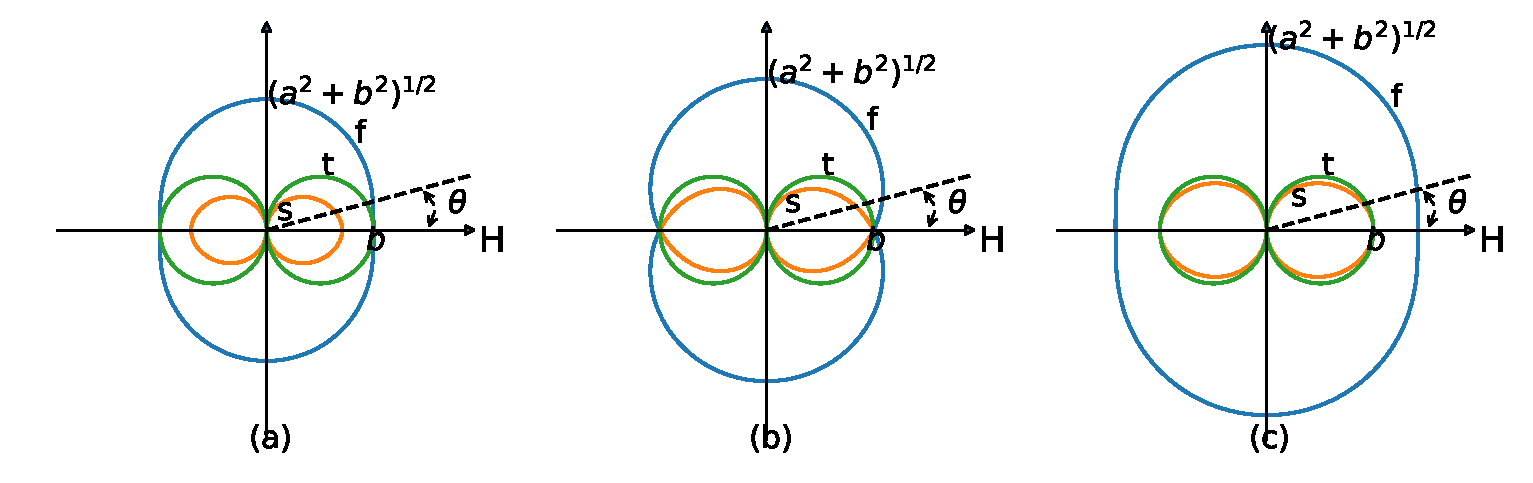
\includegraphics[width=\textwidth]{figure1.eps}
		\caption{表面法相速度图示:其中 (a) $s = 0.5$, (b) $s=1$, (c) $s=2$.}\label{Friedrich}
	\end{figure}
	
	\section{冷等离子体中的色散关系}
	
	磁化冷等离子体的色散关系可以表示为\citep{Diver2001}
	\begin{align}
		\left(S \sin^2 \theta + P \cos^2 \theta\right) n^4 - \left[R L \sin^2 \theta
		+ P S \left(1 + \cos^2 \theta\right) \right] n^2 + P R L= 0 \label{Eqn:Colp}
	\end{align}
	这里$n = k c / \omega$是折射率, $\theta$是波的传播方向和磁场的夹角,
	\begin{figure}[htb]
		%\begin{center}
		\begin{tabular}{cc}
			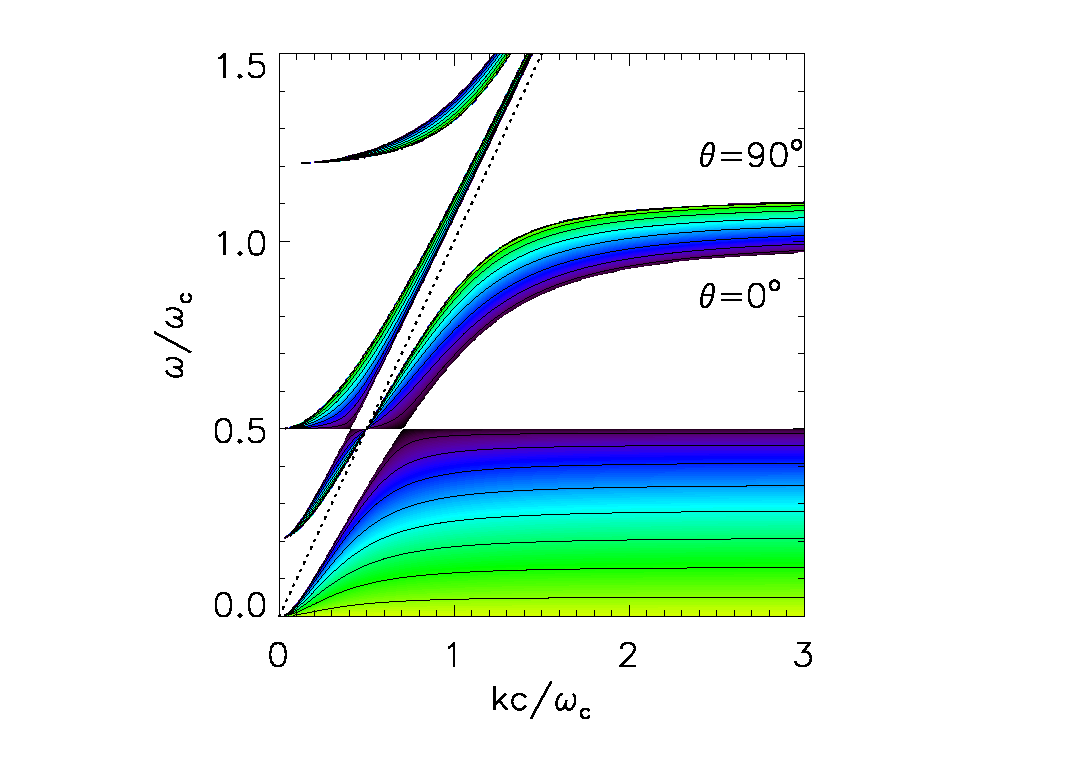
\includegraphics[scale=0.45]{figure2_2.eps} &
			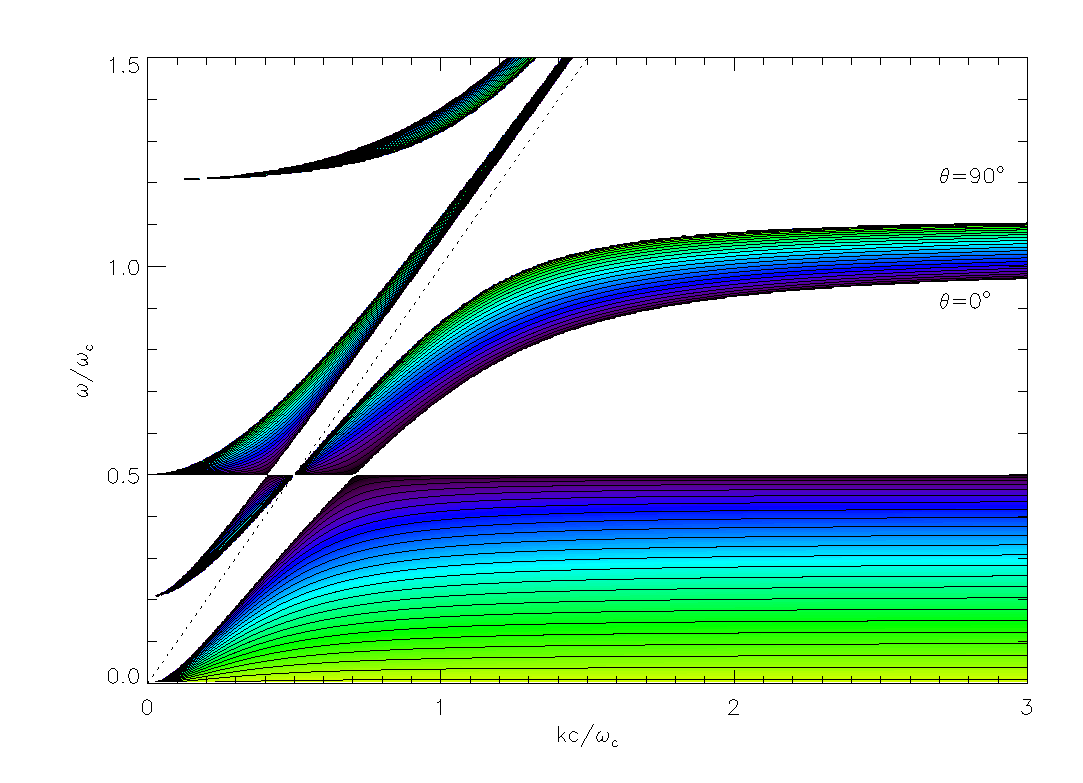
\includegraphics[scale=0.45]{figure2_1.eps}
			\\
			(a) & (b)
		\end{tabular}
		\caption{The general dispersion relation for waves in a uniform, magnetised cold
			plasma. (a) $\omega_p / \omega_c = 2.0$ and (b) $\omega_p / \omega_c = 0.5$} \label{ColdPlasma}
		%\end{center}
	\end{figure}
	\begin{align*}
		S =& (R + L) / 2
		\\
		D =& (R - L) / 2
		\\
		R =& 1 - \sum_s \frac{\omega_{ps}^2}{\omega^2} \frac{\omega}{\omega + \omega_{cs}}
		\\
		L =& 1 - \sum_s \frac{\omega_{ps}^2}{\omega^2} \frac{\omega}{\omega - \omega_{cs}}
		\\
		P =& 1 - \sum_s \frac{\omega_{ps}^2}{\omega^2}  = 1 - \frac{\omega_p^2}{\omega^2}
	\end{align*}
	其中$\omega_{ps}$ 和 $\omega_{cs}$分别是第$s$种类粒子的等离子体频率和回旋频率, $\omega_p$是整体的等离子体频率. 方程(\ref{Eqn:Colp}) 还可以写成如下的形式,
	\begin{align*}
		\tan^2 \theta = - \frac{P (n^2 - R) (n^2 - L)}{(S n^2 - R L) (n^2 - P)}.
	\end{align*}
	其中单成分的结果可以参考图\ref{ColdPlasma}为参照, 进行分析和比较.
	
	\section{磁流体力学快磁声激波关系}
	
	\begin{figure}[htb]
		\centering \large
		\begin{overpic}[scale=0.90]{figure3.pdf}
			\put(5,40){$\mathbf{\frac{X^{\pm}_f}{H_f}}$}
			\put(60,60){$\frac{X^{+}_f}{H_f}$}
			\put(75,35){$\frac{X^{-}_f}{H_f}$}
			\put(70,26){$\frac{X^{+}_f}{H_f}$}
			\put(9,5){$0$}
			\put(50,4){$\mathbf{h_f}$}
			\put(67,4){$\hat{h_f}$}
			\put(88,4){$\hat{\hat{h_f}}$}
			\put(92,23){$\frac{\left[1+s_{0}(\gamma-1)\right] \sin \theta_{0}}{\left(1-s_{0}\right)(\gamma-1)-\gamma \sin ^{2} \theta_{0}}$}
			\put(-22,23){$\frac{\sqrt{\left(1-s_{0}\right)^{2}+4 s_{0} \sin ^{2} \theta_{0}}-\left(1-s_{0}\right)}{2 \sin \theta_{0}}$}
			\put(12,26){\begin{turn}{4}
					$s_{0} \geq 1-\gamma \sin ^{2} \theta_{0} /(\gamma-1)$
				\end{turn}
			}
			\put(12,20){$s_{0} < 1-\gamma \sin ^{2} \theta_{0} /(\gamma-1)$}
			\put(66,55){\begin{sideways}
					$\rightarrow  \infty $
				\end{sideways}
			}
			\put(6,23.5){\begin{turn}{7}
					$\rightarrow$
			\end{turn}}
			\put(6,22.5){\begin{turn}{-7}
					$\rightarrow$
			\end{turn}}
		\end{overpic}
		\caption{快磁声激波关系}\label{FShock}
	\end{figure}
	
	磁流体力学快磁声激波关系中\citep{Jeffrey1964}, 用磁场增量$h_f$ ($h_f \ge 0$)
	来表示激波的强度, 通常分析下面的公式
	\begin{align}
		\frac{X_f^\pm}{h_f} = (B \pm \sqrt{R_X})/C \qquad (\ge 0) \label{Eqn:fShock}
	\end{align}
	和$h_f$的函数关系. $B$, $C$, 和 $R_X$ 由以下表达式给出,
	\begin{align}
		& B = (\gamma/2) h_f \sin\theta_0 - (1-s_0),
		\\
		& C = 2 \sin\theta_0 - (\gamma-1) h_f,
		\\
		& R_X = B^2 + C(h_f + 2 s_0 \sin\theta_0) \qquad (\ge 0).
	\end{align}
	其中$\theta_0$为波传播方向和磁场方向的夹角 ($0^\circ \le \theta_0 \le 90^\circ$),
	$\gamma=5/3$是多方指数. 讨论两种情况, 即$B$在$C$的零点
	$$
	\hat{B} \equiv B(\hat{h}_f) = \frac{\gamma}{\gamma-1} \sin^2\theta_0 - (1-s_0),
	$$
	大于等于和小于零的情况, 此处$\hat{h}_f$是$C=0$的根
	\begin{align}
		\hat{h}_f = \left(\frac{2}{\gamma-1}\right) \sin\theta_0.
	\end{align}
	具体表现为$s_0$的条件
	\begin{align}
		s_0 \ge 1 - \gamma \frac{\sin^2\theta_0}{(\gamma-1)},
	\end{align}
	和
	\begin{align}
		s_0 < 1 - \gamma \frac{\sin^2\theta_0}{(\gamma-1)}.
	\end{align}
	而$\hat{\hat{h}}_f$是$R_X = 0$的根,
	\begin{align}
		& \hat{\hat{h}}_f = \frac{1}{2(\gamma-1) - \frac{1}{2} \gamma^2 \sin^2
			\theta_0}\Big\{\sin\theta_0
		(2-\gamma)(1+s_0) \nonumber
		\\
		& \quad + 2\cos\theta_0 \sqrt{(\gamma-1)(1-s_0)^2 + s_0 \gamma^2 \sin^2\theta_0}\Big\}.
	\end{align}
	将关系(\ref{Eqn:fShock})用图形表示
	(可取$\theta_0$的某个典型值进行分析, 如$\theta_0=15^\circ$),
	并参考图\ref{FShock}或文献\citet{Jeffrey1964}第229页中的图形以进行比较.

	\section{分工说明}
	
	\begin{itemize}
		\item 毛东巍:计算并绘制图\ref{ColdPlasma},并撰写第2节相关内容;
		\item 张建: 计算并绘制图\ref{Friedrich},并撰写第1节相关内容;
		\item 钟志辉: 计算并绘制图\ref{FShock},撰写第3节相关内容,整理修改全文内容,并进行排版
	\end{itemize}
	特此说明:以上分工仅以姓名拼音为序。
	
	\section{附件}
	
	\begin{itemize}
		\item
		assign1.tex--本报告 \LaTeX 文件
		\item
		assign1.pdf--本报告PDF输出文件
		\item
		figure.py--文中第一节图\ref{Friedrich}所用的Python计算和图形绘制程序
		\item
		figure1.eps--图\ref{Friedrich}的EPS图形文件, 由Python程序生成的PS格式图形文件
		\item
		figure2.pro--文中第二节图\ref{ColdPlasma}所用的IDL计算和图形绘制程序
		\item 
		figure2\_1.eps和figure2\_2.eps--图\ref{ColdPlasma}的EPS图形文件,由IDL程序生成的PS格式图形文件.
		\item
		figure3.pro--文中第三节图\ref{FShock}所用的IDL计算和图形绘制程序
		\item 
		FShock.pdf--图\ref{FShock}的EPS图形文件,由IDL生成无公式图形,调整了边框后,使用
		\LaTeX 加注其中的公式生成.
		\item
		References.bib -- 文献文件
	\end{itemize}

	\bibliographystyle{apalike}
	\bibliography{References}
	
	
\end{document}

